\documentclass[debug,a0paper,portrait,persian]{xebaposter}

\usepackage{url}
\usepackage{amsmath}
\usepackage{amssymb}
\usepackage{relsize} % for \smaller
\usepackage{graphicx}
\usepackage{multicol}
\usepackage{xecolor}

\usepackage{wrapfig}
\graphicspath{{images/}}
\usepackage[inline]{enumitem}% for making inline list.
\setlist{noitemsep}% Save space in lists.


\usepackage{ptext}
\usepackage{xepersian}
\settextfont[Scale=1.1]{IRNazanin}

%\usepackage{geometry}
%\geometry{papersize={90cm,170cm},verbose=ture,reset}
 %%%%%%%%%%%%%%%%%%%%%%%%%%%%%%%%%%%%%%%%%%%%%%%%%%%%%%%%%%%%%%%%%%%%%%%%%%%%%%%%
 %%%% Some math symbols used in the text
 %%%%%%%%%%%%%%%%%%%%%%%%%%%%%%%%%%%%%%%%%%%%%%%%%%%%%%%%%%%%%%%%%%%%%%%%%%%%%%%%
 % Format 
% \newcommand{\RotUP}[1]{\begin{sideways}#1\end{sideways}}
 %%%%%%%%%%%%%%%%%%%%%%%%%%%%%%%%%%%%%%%%%%%%%%%%%%%%%%%%%%%%%%%%%%%%%%%%%%%%%%%%
 % Multicol Settings
 %%%%%%%%%%%%%%%%%%%%%%%%%%%%%%%%%%%%%%%%%%%%%%%%%%%%%%%%%%%%%%%%%%%%%%%%%%%%%%%%
% \setlength{\columnsep}{0.7em}
% \setlength{\columnseprule}{0mm}

%% Begin of Document
%%%%%%%%%%%%%%%%%%%%%%%%%%%%%%%%%%%%%%%%%%%%%%%%%%%%%%%%%%%%%%%%%%%%%%%%%%%%%
\begin{document}
%%% Setting User Defined Background %%%%%%%%%%%%%%%%%%%%%%%%%%%%%%%%%%%%%%%%%%%%%%%%%%
%if you want to use your preferred background, you should set background=user in poster settings.
\background{
  \begin{tikzpicture}[remember picture,overlay]%
    \fill [yellow!20] {(current page.south east) rectangle (current page.north west)};%
	\draw (current page.center)+(0pt,0pt) node[anchor=center,opacity=.1]
	{};
  \end{tikzpicture}%
} 
%%%%%%%%%%%%%%%%%%%%%%%%%%%%%%%%%%%%%%%%%%%%%%%%%%%%%%%%%%%%%%%%%%%%%%%%%%%%%
%% Here starts the poster
%%---------------------------------------------------------------------------
%% Format it to your taste with the options
%%%%%%%%%%%%%%%%%%%%%%%%%%%%%%%%%%%%%%%%%%%%%%%%%%%%%%%%%%%%%%%%%%%%%%%%%%%%%
      \definecolor{silver}{cmyk}{0,0,0,0.3}
      \definecolor{yellow}{cmyk}{0,0,0.9,0.0}
      \definecolor{reddishyellow}{cmyk}{0,0.22,1.0,0.0}
      \definecolor{black}{cmyk}{0,0,0.0,1.0}
      \definecolor{darkYellow}{cmyk}{0,0,1.0,0.5}
      \definecolor{darkSilver}{cmyk}{0,0,0,0.1}

      \definecolor{lightyellow}{cmyk}{0,0,0.3,0.0}
      \definecolor{lighteryellow}{cmyk}{0,0,0.1,0.0}
      \definecolor{lighteryellow}{cmyk}{0,0,0.1,0.0}
      \definecolor{lightestyellow}{cmyk}{0,0,0.05,0.0}

      \begin{poster}%
      % Poster Options
      {
      eyecatcher=true,
      % Color style
      bgColorOne=lightyellow,
      bgColorTwo=yellow,
      borderColor=reddishyellow,
      headerColorOne=yellow,
      headerColorTwo=reddishyellow,
%      headerFontColor=silver,
      boxColorOne=red,
      boxColorTwo=lighteryellow,
      % Format of textbox
      textborder=faded,
      % Format of text header
      headerborder=closed,
      headerheight=0.1\textheight,
      headershape=roundedleft,
      headershade=plain,
%      headerfont=\Large, %Sans Serif
      boxshade=shadetb,%plain,
      background=user,%plain,
      linewidth=2pt,
      grid=false,
      }
 % Eye Catcher
 {
      
\includegraphics[height=0.07\textheight]{utlogo}
 }
 % Title
 {حفظ حریم زمانی  در شبکه‌های ارتباطی با استفاده از تئوری صف 
}
 % Authors
 {\large ابوالفضل دیانت 
 \\%[1em]
 {\normalsize\texttt{\lr{ab.diyanat@gmail.com}}}}
 % University logo
 {
\begin{tabular}{r}
 %   
\includegraphics[height=0.04 \textheight]{utlogo}\\
\end{tabular}
 }

%%%%%%%%%%%%%%%%%%%%%%%%%%%%%%%%%%%%%%%%%%%%%%%%%%%%%%%%%%%%%%%%%%%%%%%%%%%%%%
%%% Now define the boxes that make up the poster
%%%---------------------------------------------------------------------------
%%% Each box has a name and can be placed absolutely or relatively.
%%% The only inconvenience is that you can only specify a relative position 
%%% towards an already declared box. So if you have a box attached to the 
%%% bottom, one to the top and a third one which should be inbetween, you 
%%% have to specify the top and bottom boxes before you specify the middle 
%%% box.
%%%%%%%%%%%%%%%%%%%%%%%%%%%%%%%%%%%%%%%%%%%%%%%%%%%%%%%%%%%%%%%%%%%%%%%%%%%%%%

 %%%%%%%%%%%%%%%%%%%%%%%%%%%%%%%%%%%%%%%%%%%%%%%%%%%%%%%%%%%%%%%%%%%%%%%%%%%%%%
\begin{posterbox}[name=introduction,column=0,row=0]{\textxecolor{red}{مقدمه}}
 %%%%%%%%%%%%%%%%%%%%%%%%%%%%%%%%%%%%%%%%%%%%%%%%%%%%%%%%%%%%%%%%%%%%%%%%%%%%%%
امنیت از مهم‌ترین واژه‌هایی است که در فکر و ذهن بشر، از نخستین لحظات زندگانی‌اش در جریان بوده‌است. هنگامی که  ژولیوس سزار‎‎
برای نخستین بار در ۵۰ سال قبل از میلاد، رمز ساده جانشینی حرفی خود را بکار گرفت، هیچ‌گاه فکر نمی‌کرد که حوزه‌ای که در آن گام نهاده، به یکی از بزرگترین حوزه‌های تحقیقاتی دنیا مبدل خواهد شد.  امنیت در حوالی جنگ جهانی دوم رشد شگرفی را تجربه کرد. اما آن‌چه که ما اکنون بر  آن گام می‌نهیم، مدیون دو انقلاب  بزرگ در این حوزه است، مقاله ۱۹۴۹ شانون
\lr{Claude Elwood Shannon (April 30, 1916 – Feb 24, 2001)}
 و دیگری بوجود آمدن مفهوم امنیت مبتنی بر کلید عمومی
(\lr{Public Key}).

تا مدت‌ها نگاه ما به امنیت به سه‌گانه
\lr{CIA}
خلاصه می‌گشت، اما با گذر زمان مفاهیم جدیدی نظیر تازگی، انکارناپذیری، گمنامی و حفظ حریم خصوصی نیز مطرح گشت و جای خود را در این حوزه پیدا کرد. در این مجال، از دریای بی‌کران امنیت، به سراغ حفظ حریم‌خصوصی می‌رویم
\cite{menezes1996handbook}.




\end{posterbox}
 %%%%%%%%%%%%%%%%%%%%%%%%%%%%%%%%%%%%%%%%%%%%%%%%%%%%%%%%%%%%%%%%%%%%%%%%%%%%%%
\begin{posterbox}[name=phase2,column=1,span=1]{کاربردها}
\textbf{۱- طبقه‌بندی ترافیک}

\centerline{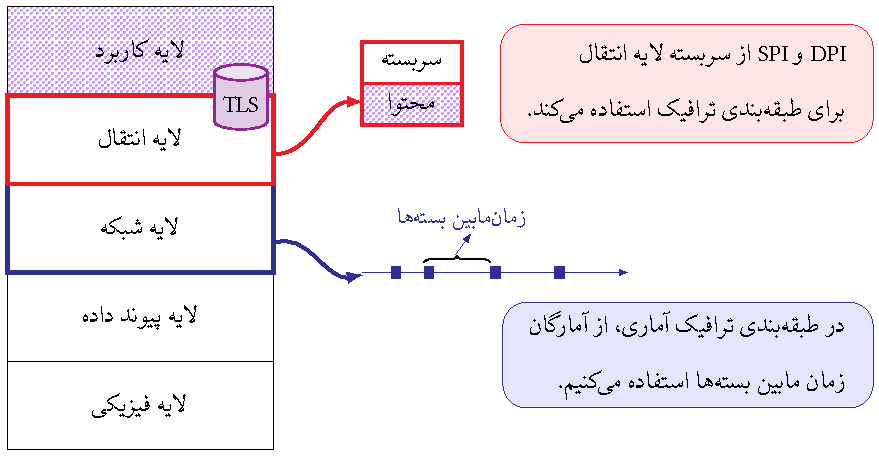
\includegraphics[width=\linewidth]{images/networkLayer}}


\textbf{2 - شبکه‌های حسگر بی‌سیم}

\centerline{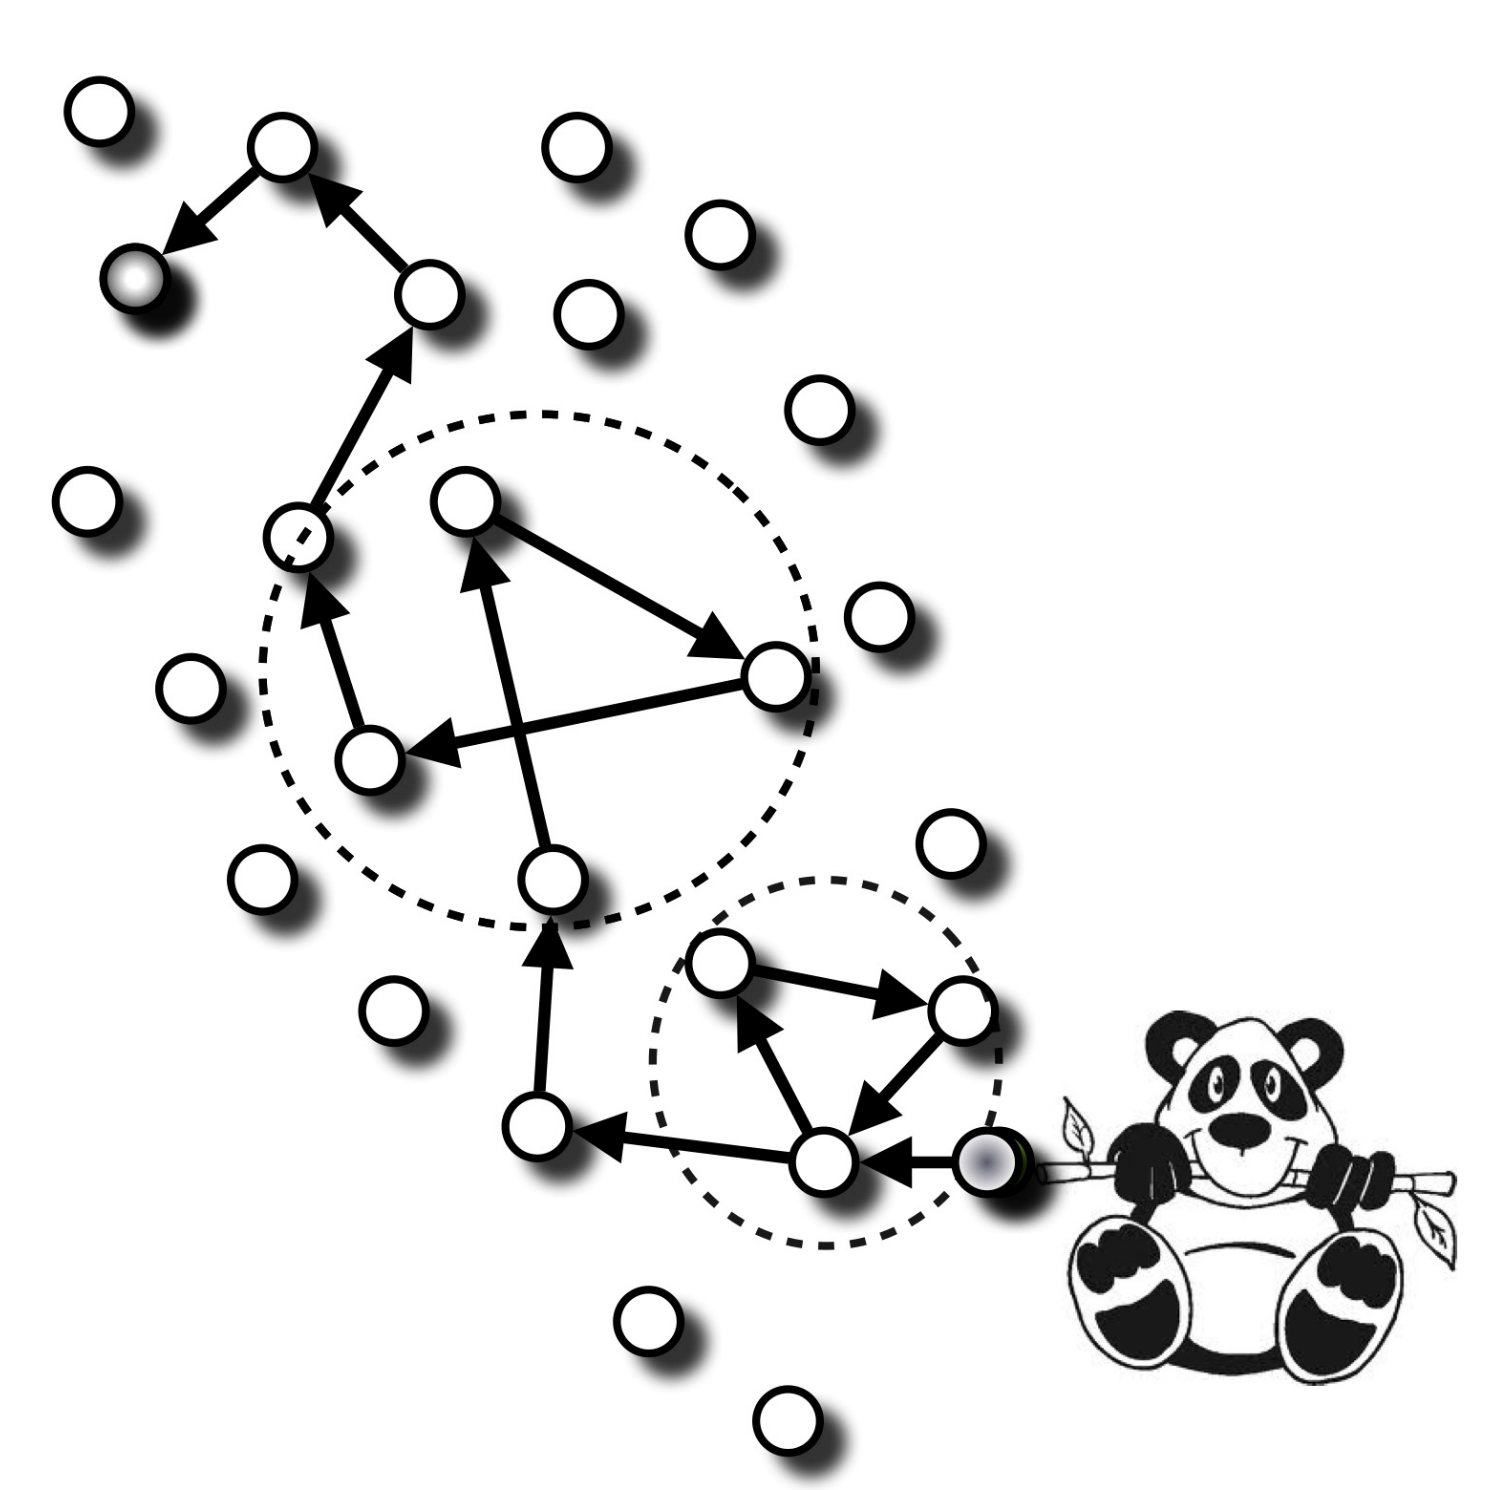
\includegraphics[width=\linewidth]{images/panda2}}

\textbf{3 - \lr{WBAN}}

\centerline{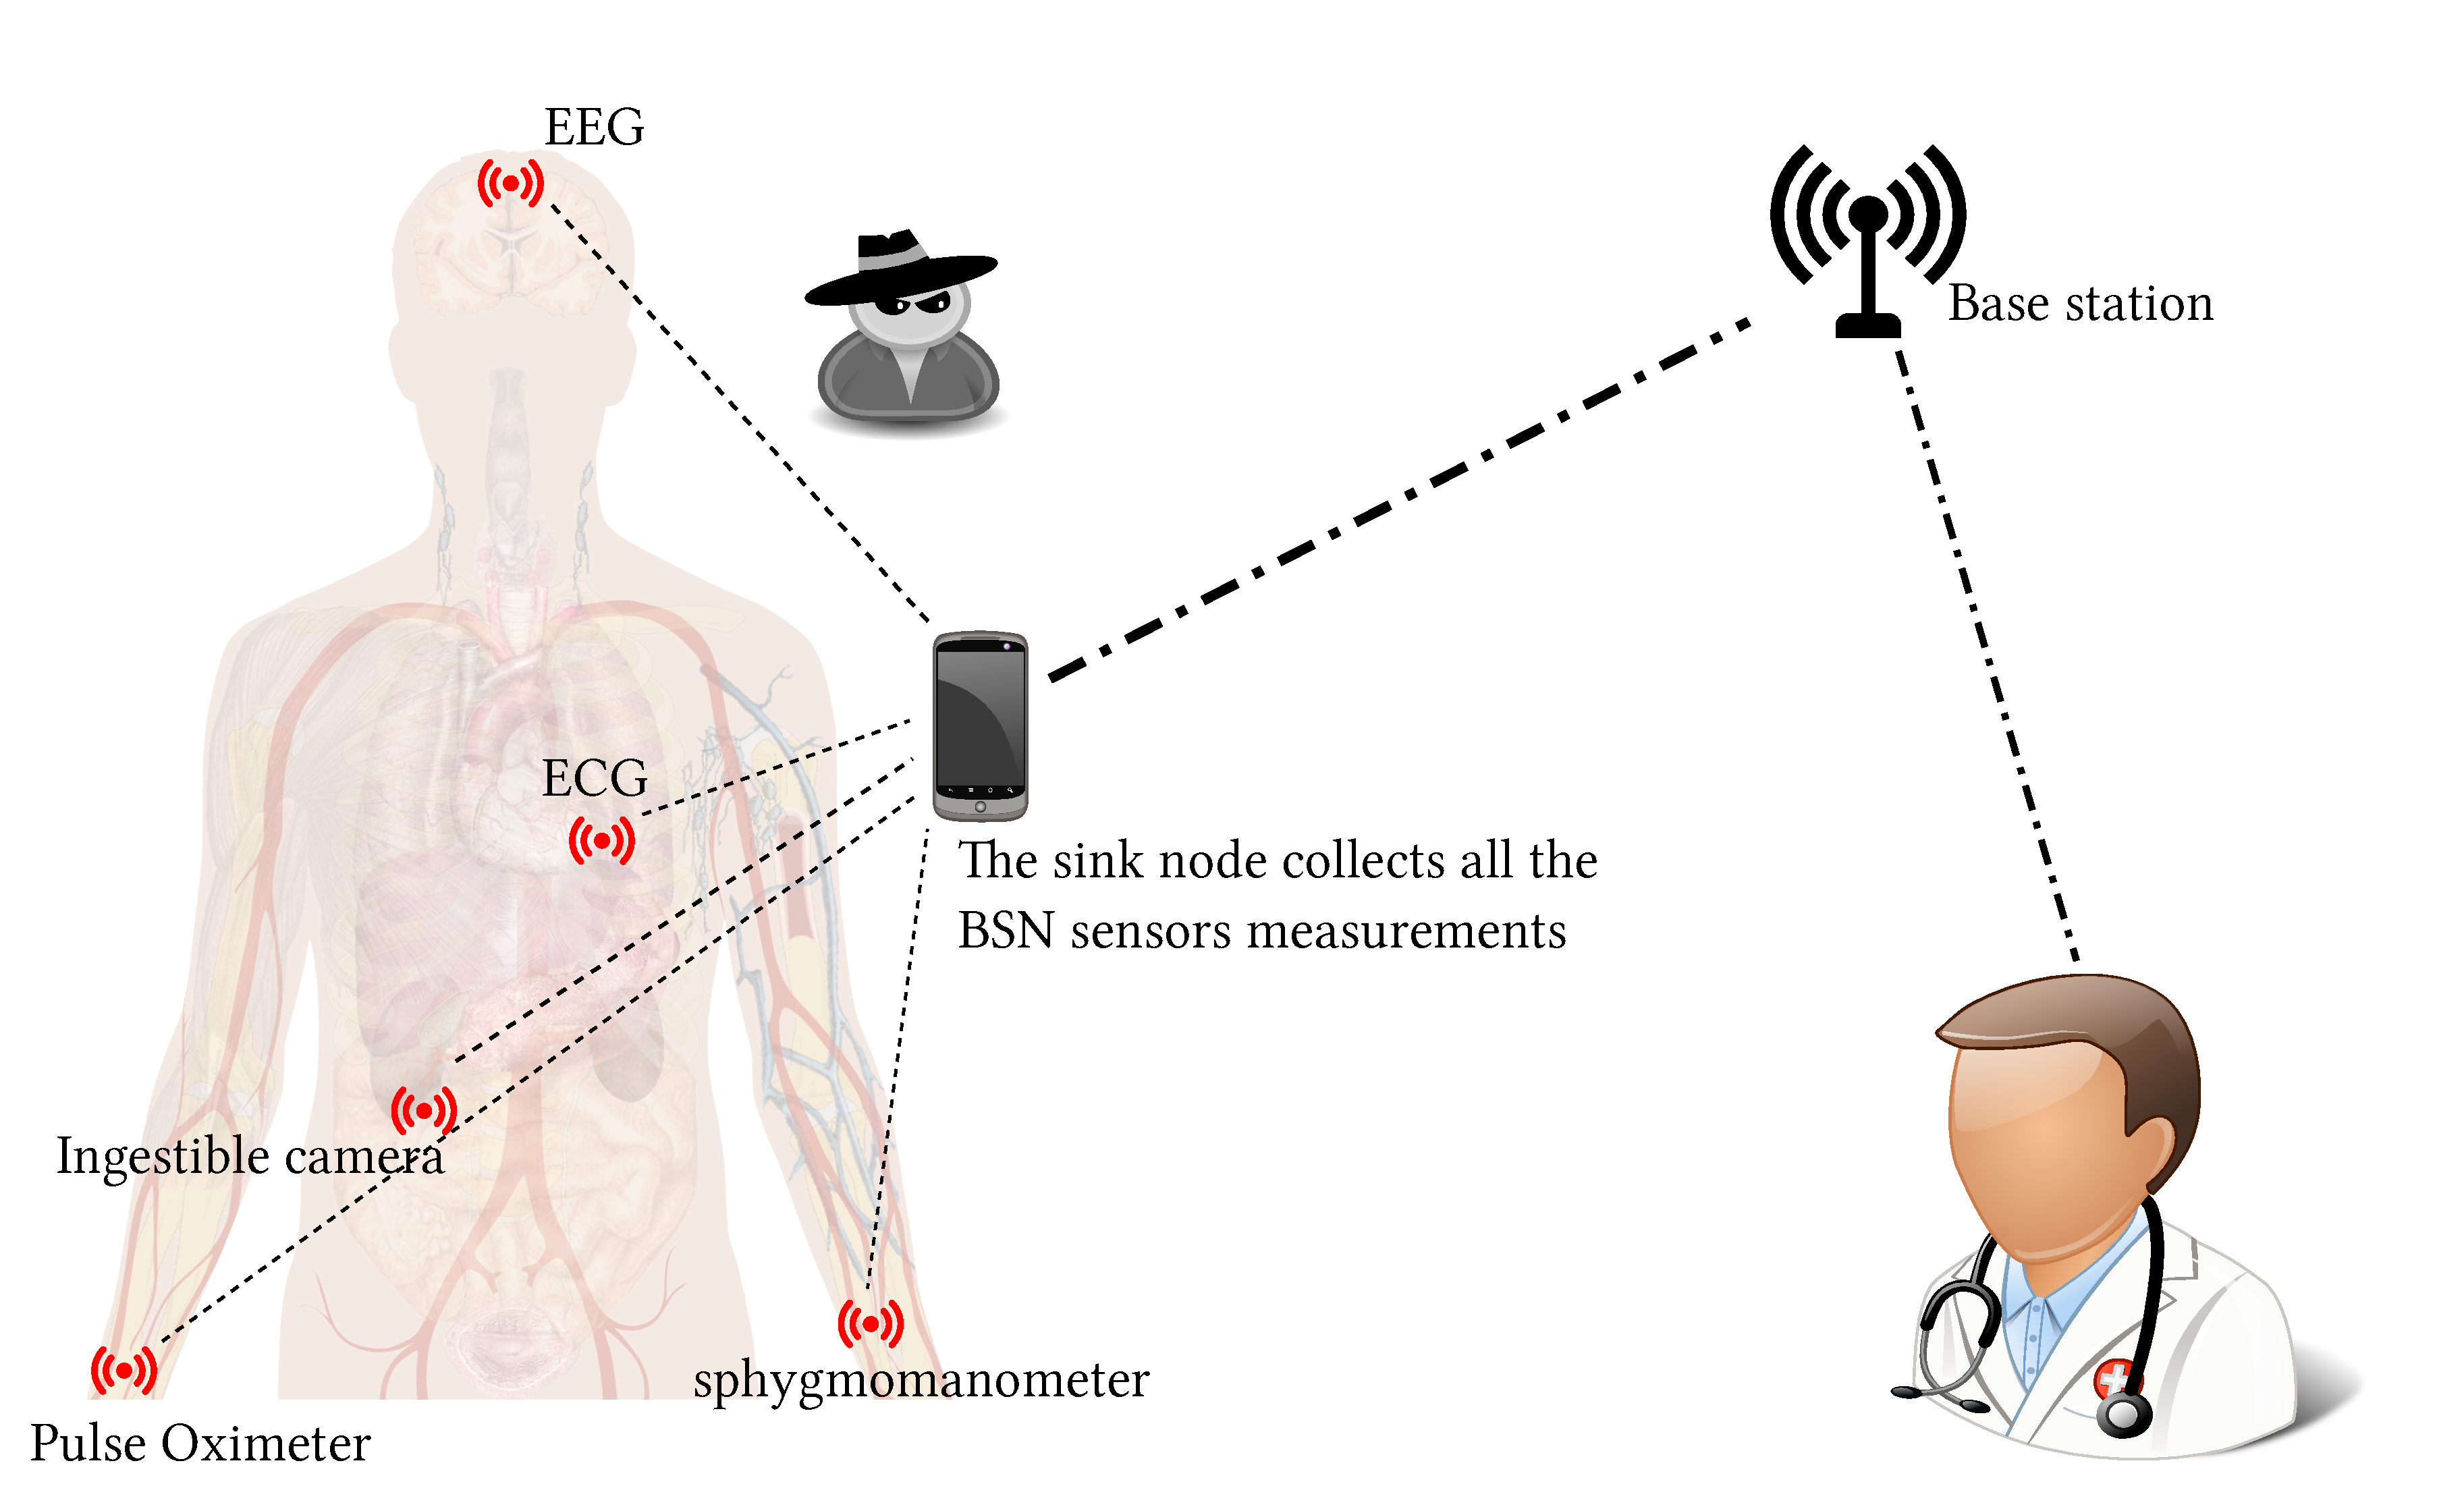
\includegraphics[width=\linewidth]{images/WBAN}}

\textbf{4 - تشخیص ناهنجاری} 

  \centerline{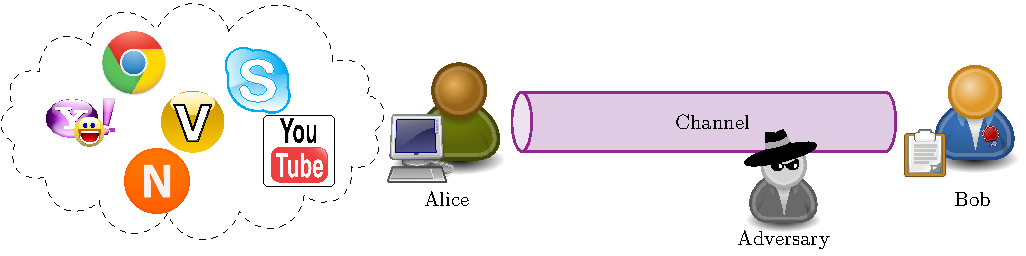
\includegraphics[width=\linewidth]{images/AliceOperatorBobExt}}

\textbf{۵ - سامانه‌های ذخیره‌سازی} 

  \centerline{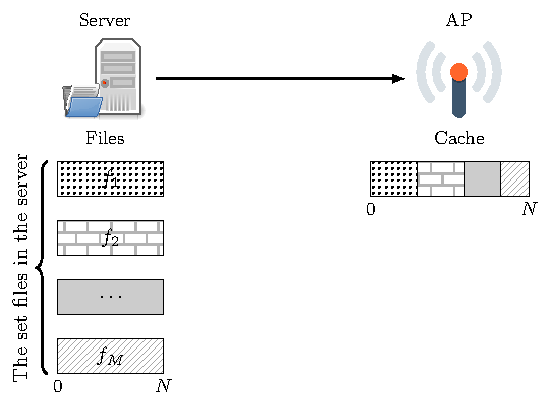
\includegraphics[width=\linewidth]{images/CachingSystem}}

\end{posterbox}

 %%%%%%%%%%%%%%%%%%%%%%%%%%%%%%%%%%%%%%%%%%%%%%%%%%%%%%%%%%%%%%%%%%%%%%%%%%%%%%
\begin{posterbox}[name=phase3,column=2,span=1,row=0]{مثال انگیزه‌بخش}
  \centerline{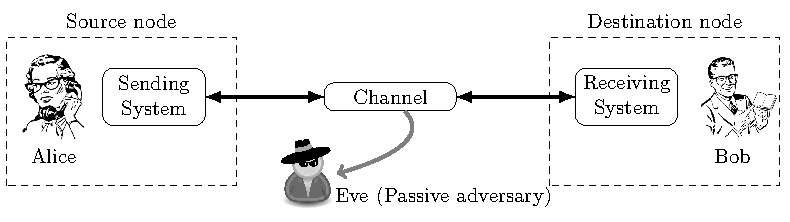
\includegraphics[width=\linewidth]{images/SystemTotalStoryWithCharacter}}


\lr{Alice} (گره مبدا)
قصد تبادل اطلاعات با
\lr{Bob} (گره مقصد)
را دارد. فرض کنید که
\lr{Alice}
در هر بازه زمانی، یک کاربرد از مجموعه هفت کاربرد موجود بر روی سامانه خود را اجرا می‌کند. اجازه دهید که نرخ تولید بسته‌ها توسط 
کاربرد $i$ام 
($1\leq i \leq 7$) را با $\lambda_g^i\in \Lambda_g$
نشان دهیم، که 
$\Lambda_g$
بیانگر مجموعه‌ نرخ‌های این هفت کاربرد است. در ادامه  $\Lambda_g$ را به صورت زیر در نظر بگیرید. 
\begin{equation*}
\Lambda_g = \{100, 230, 350, 400, 480, 520, 610\}\;[\mathrm{kbps}].
\end{equation*}
در این میان
\lr{Eve}
به عنوان یک مهاجم، به شنود کانال ارتباطی بین
\lr{Alice} و \lr{Bob}
می‌پردازد. او قصد دارد بداند که 
\lr{Alice}
کدام یک از این هفت کاربرد را در آن بازه زمانی اجرا نموده است. به دلیل استفاده از سازوکارهای امنیتی (نظیر رمزنگاری)
 به نظر می‌رسد \lr{Eve} نتواند به محتوای بسته‌های
ارسالی دست یابد و به ناچار دست به دامان  قانون پایستگی جریان
(\lr{Flow Conservation Law}) \cite[قضیه 3.4.5]{Kesidis2007Introduction}
می‌شود. برطبق این قانون نرخ خروج بسته‌های ارسالی از سوی 
\lr{Alice}،
برابر با نرخ تولید بسته‌ها خواهد بود. بدین‌سان و با علم به  نگاشت هر نرخ به کاربرد متناظرش، می‌تواند  به مقصود خود نایل گردد.

به دنبال آن هستیم که راه‌کاری پیش پای \lr{Alice} برای حفظ حریم‌خصوصی نرخ بگذاریم. خواهید دید که اضافه کردن بسته‌های
\lr{Dummy}
جزو مواردی است که قانون پایستگی جریان را نقض می‌کند. بدین‌سان 
\lr{Alice}
برای حفظ حریم‌خصوصی کاربرد 
$i$  با نرخ $\lambda_g^i$،
سعی می‌کند با اضافه کردن جریانی از بسته‌ها با نرخ  
$\lambda_d^{ij}=\lambda_g^j-\lambda_g^i$،
نرخ بسته‌های خروجی را به 
$\lambda_g^j$
برساند، به طوری که 
$\lambda_g^j\in \Lambda_g$.

\centerline{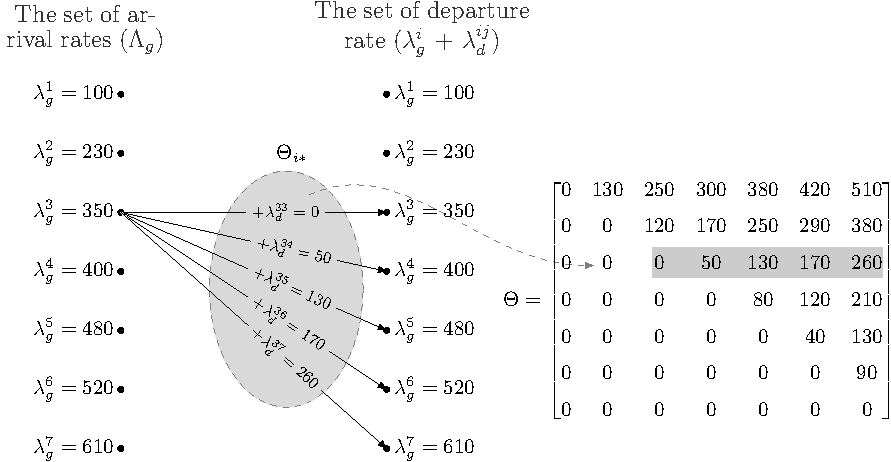
\includegraphics[width=\linewidth]{images/mappingTable}}


\end{posterbox}
\begin{posterbox}[name=results,column=2,span=1,below=phase3]{نوآوری}
\textbf{درجه حریم‌خصوصی}:
به احتمال خطای بهترین تخمین مهاجم  از  شناسه کاربرد، درجه حریم‌خصوصی گره مبدا می‌گوییم. 

ذکر خواهد شد که نامساوی \lr{Fano}
 \cite[قضیه $2.10.1$]{cover2006elements}
ما را یاری می‌رساند تا بتوانیم یک کران پایین برای خطای مهاجم
($P_e$) در بهترین تخمینش 
بیابیم.
\begin{itemize}
\item 
ارایه یک روش پیشنهادی (اضافه نمودن بسته‌های ساختگی) به صورت کامل ارایه خواهد شد.  

\item
توصیف رفتار ‎\lr{Alice}‎ در اضافه نمودن بسته‌های  ساختگی، مبتنی بر یک مدل ریاضیاتی بر مبنای 
\lr{Preemptive Resume Priority Queue}. 
\item
 شروطی نیز بر روی نحوه ارسال بسته‌های ساختگی، چراکه اضافه‌کردن بسته‌های ساختگی، ممکن است موجب سوق‌ داده شدن سامانه به ناحیه غیرپایدار است. 
\end{itemize}
\end{posterbox}


%%%%%%%%%%%%%%%%%%%%%%%%%%%%%%%%%%%%%%%%%%%%%%%%%%%%%%%%%%%%%%%%%%%%%%%%%%%%%%
\begin{posterbox}[name=imagedataset,column=0,span=1,below=introduction]{امنیت مبتنی بر اطلاعات جانبی}
حفظ‌ حریم‌خصوصی در دو دسته
\cite[صفحه 202]{mason2014sensing}:
\begin{itemize}
\item 
 مبتنی بر داده
(\lr{Data Oriented})
\item
مبتنی بر اطلاعات جانبی
(\lr{ContextOriented})
\end{itemize}
نقطه تمرکز حریم‌خصوصی مبتنی بر  داده، بر روی محتوای داده است و بدین‌سان سازوکارهایی نظیر رمزنگاری و حفظ یکپارچگی برای تامین چنین نیازی کارا و کافی خواهد بود. در حریم‌خصوصی مبتنی بر اطلاعات جانبی، هدف غایی کسب اطلاعات جانبی  از داده‌ها است. فرض کنید جلسه‌ای محرمانه بین دو نفر تشکیل شده است. در این نوع از  حفظ حریم‌خصوصی، محتوای داده (صحبت‌هایی که در جلسه مطرح شده) برای ما اهمیت ندارد، بلکه اطلاعات جانبی آن نظیر  این‌که چه‌کسانی، درکجا، کی، چگونه و چرا این جلسه را برگزار کردند، از اهمیت بیشتری برخوردار خواهد بود. 

آن‌چه که ما به دنبال آن هستیم، نوعی از حریم‌خصوصی است که ما آن را حریم‌خصوصی زمانی و آماری
(\lr{Temporal and Statistical Privacy})
می‌نامیم. این نوع از حریم‌خصوصی،  هر نوع اطلاعاتی از زمان رخداد یک حادثه چه به صورت قطعی و چه به صورت آماری (به عنوان نمونه
نرخ و پراش زمان رخداد آن حادثه)  ممکن است حریم‌خصوصی کاربر را به مخاطره بیافکند.
\vskip 3mm
  \centerline{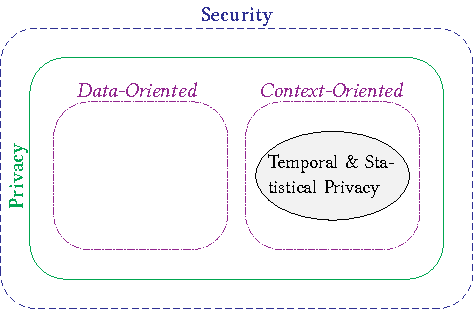
\includegraphics[width=.9\linewidth]{images/WhatInThesis}}

حفظ حریم زمانی و آماری از جنبه‌های بسیاری می‌تواند حائز اهمیت باشد. ما در نقش پدآفندی قرار داریم. 


\end{posterbox}
 %%%%%%%%%%%%%%%%%%%%%%%%%%%%%%%%%%%%%%%%%%%%%%%%%%%%%%%%%%%%%%%%%%%%%%%%%%%%%%

%%%%%%%%%%%%%%%%%%%%%%%%%%%%%%%%%%%%%%%%%%%%%%%%%%%%%%%%%%%%%%%%%%%%%%%%%%%%%%

%%%%%%%%%%%%%%%%%%%%%%%%%%%%%%%%%%%%%%%%%%%%%%%%%%%%%%%%%%%%%%%%%%%%%%%%%%%%%%
\begin{posterbox}[name=references,column=0,span=3,below=phase2]{منابع}
 %%%%%%%%%%%%%%%%%%%%%%%%%%%%%%%%%%%%%%%%%%%%%%%%%%%%%%%%%%%%%%%%%%%%%%%%%%%%%%
     \smaller
%     \bibliographystyle{ieee}
     \renewcommand{\section}[2]{\vskip 0.05em}
\bibliographystyle{ieeetr-fa}
\bibliography{library}
\end{posterbox}
 
\end{poster}

\end{document}
